\chapter{Arhitektura i dizajn sustava}
		
		\textbf{\textit{dio 1. revizije}}\\

		\textit{ Potrebno je opisati stil arhitekture te identificirati: podsustave, preslikavanje na radnu platformu, spremišta podataka, mrežne protokole, globalni upravljački tok i sklopovsko-programske zahtjeve. Po točkama razraditi i popratiti odgovarajućim skicama:}
	\begin{itemize}
		\item 	\textit{izbor arhitekture temeljem principa oblikovanja pokazanih na predavanjima (objasniti zašto ste baš odabrali takvu arhitekturu)}
		\item 	\textit{organizaciju sustava s najviše razine apstrakcije (npr. klijent-poslužitelj, baza podataka, datotečni sustav, grafičko sučelje)}
		\item 	\textit{organizaciju aplikacije (npr. slojevi frontend i backend, MVC arhitektura) }		
	\end{itemize}

			

				
		\section{Baza podataka}
			
			\textbf{\textit{dio 1. revizije}}\\			
		
			
				\noindent Za potrebe našeg sustava koristit ćemo relacijsku bazu podataka koja svojom strukturom olakšava modeliranje stvarnog svijeta. Temeljna jedinica baze je relacija, odnosno tablica koja je definirana svojim imenom i skupom atributa. Glavna svrha baze podataka je brza i jednostavna pohrana, izmjena i dohvaćanje podataka za daljnju obradu. Baza podataka ove aplikacije sastoji se od sljedećih entiteta:
				
				\begin{itemize}
					\item USER
					\item RESEARCHER
					\item MANAGER
					\item TRACKER
					\item ANIMAL
					\item STATION
					\item ACTION
					\item TASK
					\item MEDIUM
					\item QUALIFICATION
					\item TRACKER\_IN\_ACTION
					\item TRACKER\_IN\_ACTION\_ARCHIVE
					\item TRACKER\_LOCATION
					\item ANIMAL\_LOCATION
					\item STATION\_LOCATION
					\item TRACKER\_HISTORY
					\item ANIMAL\_HISTORY
					\item ROUTE
					\item ROUTE\_POINT\_LOCATION
					\item ANIMAL\_COMMENT
					\item MAP\_COMMENT
				\end{itemize}
				
		\subsection{Opis tablica}
				
				
				\noindent \textbf{USER} \hspace{1em} Ovaj entitet sadržava sve važne informacije vezane za korisnika aplikacije. Sadrži atribute ID korisnika, korisničko ime korisnika u aplikaciji, fotografiju korisnika, šifru računa korisnika, pravo ime i prezime korisnika, e-mail adresu i atribut koji označava je li korisnik registriran tipa BOOL.  Ova klasa sadrži zajedničke atribute sva tri tipa korisnika aplikacije (voditelj, istraživač, tragač) te služi za lakše spremanje podataka koje svaki korisnik mora imati. Ovaj entitet je  vezi \textit{One-to-One} sa svakim tipom korisnika aplikacije. S klasom MAP\_COMMENT je u vezi \textit{One-to-Many} jer više korisnika (mora biti istraživač ili tragač) može ostaviti komentar na mapi.
				
				
				\begin{longtblr}[
					label=none,
					entry=none
					]{
						width = \textwidth,
						colspec={|X[6,l]|X[6, l]|X[20, l]|}, 
						rowhead = 1,
					} %definicija širine tablice, širine stupaca, poravnanje i broja redaka naslova tablice
					\hline \SetCell[c=3]{c}{\textbf{USER}}	 \\ \hline[3pt]
					\SetCell{LightGreen}id & INT	&  	jedinstveni identifikator (TRACKER.id ili MANAGER.id ili RESEARCHER.id)  	\\ \hline
					username & VARCHAR &   korisničko ime 	\\ \hline 
					photo & PHOTOTYPE & fotografija korisnika 	\\ \hline
					password & VARCHAR	& šifra korisničkog računa \\ \hline
					name & VARCHAR	& ime korisnika \\ \hline
					surname & VARCHAR & prezime korisnika \\ \hline
					email & VARCHAR & e-mail korisnika  \\ \hline 
					registered & BOOL & oznaka koja definira je li korisnik registriran  \\ \hline
				\end{longtblr}
				
				
				\noindent \textbf{RESEARCHER} \hspace{1em} Ovaj entitet sadrži dodatni atribut odobrenja koji je potreban korisniku koji se odlučio za ulogu istraživača u aplikaciji. Povezan je s klasom USER vezom \textit{One-to-One} preko ID ključa. Dodatni atribut nam govori je li korisnik odobren kao istraživač od strane administratora jer je to preduvjet za obavljanje te uloge. U vezi je \textit{One-to-Many} s klasom ACTION (svaki istraživač može organizirati više radnih akcija). S klasom MAP\_COMMENT je indirektno (pomoću USER.id) u vezi \textit{One-to-Many} jer više korisnika može ostaviti komentar na mapi.
				
				\begin{longtblr}[
					label=none,
					entry=none
					]{
						width = \textwidth,
						colspec={|X[6,l]|X[6, l]|X[20, l]|}, 
						rowhead = 1,
					} %definicija širine tablice, širine stupaca, poravnanje i broja redaka naslova tablice
					\hline \SetCell[c=3]{c}{\textbf{RESEARCHER}}	 \\ \hline[3pt]
					\SetCell{LightGreen}id & INT &	identifikator istraživača (USER.id)	\\ \hline
					approved & BOOL & oznaka je li istraživač odobren od strane administratora\\ \hline
				\end{longtblr}				
				
				
				\noindent \textbf{MANAGER} \hspace{1em} Ovaj entitet sadrži dodatne atribute koji opisuju korisnika koji ima ulogu voditelja neke stanice. Moguće je da voditelj vodi samo jednu stanicu i također da jedna stanica ima samo jednog voditelja i zato je veza klase STATION i MANAGER \textit{One-to-One}. Dodatni atribut approved  označava je li korisniku odobren zahtjev za ulogu voditelja od strane administratora (isto kao kod istraživača) te atribut idStation označava jedinstveni identifikator stanice kojoj je korisnik voditelj.
				
				
				\begin{longtblr}[
					label=none,
					entry=none
					]{
						width = \textwidth,
						colspec={|X[6,l]|X[6, l]|X[20, l]|}, 
						rowhead = 1,
					} %definicija širine tablice, širine stupaca, poravnanje i broja redaka naslova tablice
					\hline \SetCell[c=3]{c}{\textbf{MANAGER}}	 \\ \hline[3pt]
					\SetCell{LightGreen}id & INT & jedinstveni identifikator (USER.id) \\ \hline
					approved & BOOL & oznaka odobrenja \\ \hline
					\SetCell{LightBlue}idStation & INT & identifikator stanice (STATION.id) \\ \hline
				\end{longtblr}
				
				
				\noindent \textbf{TRACKER} \hspace{1em} Ovaj entitet označava korisnika koji obavlja ulogu tragača. Povezan je vezama \textit{One-to-One} s klasom USER i klasom TRACKER\_IN\_ACTION koja označava tragača koji trenutno obavlja zadatke neke akcije i vozilo kojim se koristi, te vezom \textit{Many-to-One} s klasom STATION i vezom \textit{One-to-Many} s klasom TASK jer jedan tragač može imati više zadataka te klasom TRACKER\_IN\_ACTION\_ARCHIVE koja čuva podatke o tragačima koji su sudjelovali u nekoj akciji. Tragač može obavljati zadatke koji su zadani od strane istraživača samo na jednoj stanici, dok stanica može imati više tragača na različitim zadatcima. S klasom ANIMAL\_COMMENT je u vezi \textit{One-to-Many} jer više tragača može ostaviti komentar na nekoj životinji te je također u vezi \textit{One-to-One} s klasom TRACKER\_LOCATION koja služi za čuvanje lokacija tragača.  Također je u vezi \textit{Many-to-Many} s klasom MEDIUM što se razrješava tablicom QUALIFICATION. S klasom MAP\_COMMENT je indirektno (pomoću USER.id) u vezi \textit{One-to-Many} jer više korisnika može ostaviti komentar na mapi.
				
				\begin{longtblr}[
					label=none,
					entry=none
					]{
						width = \textwidth,
						colspec={|X[6,l]|X[6, l]|X[20, l]|}, 
						rowhead = 1,
					} %definicija širine tablice, širine stupaca, poravnanje i broja redaka naslova tablice
					\hline \SetCell[c=3]{c}{\textbf{TRACKER}}	 \\ \hline[3pt]
					\SetCell{LightGreen}id & INT & jedinstveni identifikator tragača (USER.id) \\ \hline
					\SetCell{LightBlue} idStation & INT & jedinstveni identifikator stanice (STATION.id)\\ \hline
				\end{longtblr}
				
				\noindent \textbf{ANIMAL} \hspace{1em} Ovaj entitet predstavlja klasu životinja i sadrži sve atribute koji opisuju neku životinju. Sadrži atribute ID životinje, vrstu životinje, fotografiju životinje, tekst koji opisuje životinju i oznaku koja govori je li postavljen GPS na životinju ili nije. U vezi je \textit{One-to-Many} s klasom  TASK jer na nekom zadatku se može pratiti jedna životinja dok više zadataka može pratiti istu životinju. S klasom ANIMAL\_COMMENT je u vezi \textit{One-to-Many} jer više komentara se može ostaviti za istu životinju. Također je u vezi \textit{One-to-One} s klasom ANIMAL\_LOCATION koja zapisuje trenutnu lokaciju životinje, ali je u vezi \textit{One-to-Many} s klasom ANIMAL\_HISTORY koja sprema podatke o kretanju životinje.
				
				
				\begin{longtblr}[
					label=none,
					entry=none
					]{
						width = \textwidth,
						colspec={|X[6,l]|X[6, l]|X[20, l]|}, 
						rowhead = 1,
					} %definicija širine tablice, širine stupaca, poravnanje i broja redaka naslova tablice
					\hline \SetCell[c=3]{c}{\textbf{ANIMAL}}	 \\ \hline[3pt]
					\SetCell{LightGreen}id & INT & jedinstveni identifikator \\ \hline
					species & VARCHAR & vrsta životinje \\ \hline
					photo & PHOTOTYPE & fotografija životinje \\ \hline
					description & TEXT & opis životinje \\ \hline
					hasGPS & BOOL & potvrda GPS uređaja na životinji \\ \hline
				\end{longtblr}
				
				
				
				\noindent \textbf{STATION} \hspace{1em} Ovaj entitet predstavlja klasu stanice koja sadrži atribute koje opisuju stanicu; ID stanice, ime stanice te kratki opis stanice. U vezi je \textit{One-to-One} s klasom STATION\_LOCATION koja sadrži podatke o lokaciji stanice i s klasom MANAGER jer je za svaku stanicu zadužen je točno jedan voditelj te je u vezi \textit{One-to-Many} s klasom TRACKER jer više tragača može raditi za istu stanicu.
				
				\begin{longtblr}[
					label=none,
					entry=none
					]{
						width = \textwidth,
						colspec={|X[6,l]|X[6, l]|X[20, l]|}, 
						rowhead = 1,
					} %definicija širine tablice, širine stupaca, poravnanje i broja redaka naslova tablice
					\hline \SetCell[c=3]{c}{\textbf{STATION}}	 \\ \hline[3pt]
					\SetCell{LightGreen}id & INT & jedinstveni identifikator stanice \\ \hline
					name & VARCHAR & ime stanice \\ \hline
					description & TEXT & opis stanice \\ \hline
				\end{longtblr}
				
				
				\noindent \textbf{ACTION} \hspace{1em} Ovaj entitet sadržava sve važne informacije vezane za akciju koju provodi određeni istraživač. Sadrži atribute ID, naslov, ID istraživača koji provodi akciju, vrijeme početka, vrijeme kraja te status koji je kodni broj za trenutno stanje akcije (čeka da postane aktivna, aktivna, riješena, prekinuta). Ovaj entitet u vezi je \textit{Many-to-One} s entitetom RESEARCHER preko ID-a istraživača te je u vezi \textit{One-to-Many} s entitetima TASK koji predstavlja zadatak, TRACKER\_IN\_ACTION koji predstavlja trenutno aktivne tragače u akcijama te njihov način prijevoza, TRACKER\_IN\_ACTION\_ARCHIVE koji predstavlja prošle zapise tragača aktivnih na akcijama te njihov način prijevoza, ANIMAL\_COMMENT koji predstavlja komentar tragača vezan za određenu životinju u nekoj akciji, MAP\_COMMENT koji predstavlja komentar vezan za određenu lokaciju u nekoj akciji te ga mogu napisati istraživač ili tragač.
				
				\begin{longtblr}[
					label=none,
					entry=none
					]{
						width = \textwidth,
						colspec={|X[6,l]|X[6, l]|X[20, l]|}, 
						rowhead = 1,
					} %definicija širine tablice, širine stupaca, poravnanje i broja redaka naslova tablice
					\hline \SetCell[c=3]{c}{\textbf{ACTION}}	 \\ \hline[3pt]
					\SetCell{LightGreen}id & INT & jedinstveni identifikator \\ \hline
					title & VARCHAR & naslov akcije \\ \hline
					\SetCell{LightBlue}idResearcher & INT & ID istraživača (RESEARCHER.id) \\ \hline
					start & TIMESTAMP & vrijeme početka \\ \hline
					end & TIMESTAMP & vrijeme kraja \\ \hline
					status & INT & kodni broj za trenutno stanje akcije \\ \hline
				\end{longtblr}
				
				
				\noindent \textbf{TASK} \hspace{1em} Ovaj entitet sadržava sve važne informacije vezane za zadatak koji je dio neke akcije te ga odrađuje određeni tragač. Sadrži atribute ID, naslov, ID tragača koji odrađuje zadatak, ID akcije kojoj pripada, ID životinje u slučaju da je zadatak da se prati neku životinju, vrsta životinje u slučaju da je zadatak povezan s nekom vrstom životinje, geografska širina i dužina za slučaj da je potrebno otići na neku lokaciju, ID rute za slučaj da je potreban prolazak nekom rutom, površina za slučaj da je potrebno istražiti neku površinu, sadržaj u kojem je opisan zadatak, vrijeme početka, vrijeme kraja te status koji je kodni broj za trenutno stanje zadatka (čeka da postane aktivan, aktivan, riješen, prekinut). Ovaj entitet u vezi je \textit{Many-to-One} s entitetima RESEARCHER preko ID-a istraživača, ACTION preko ID-a akcije, ANIMAL preko ID-a životinje, ROUTE preko ID-a rute.
				
				\begin{longtblr}[
					label=none,
					entry=none
					]{
						width = \textwidth,
						colspec={|X[6,l]|X[6, l]|X[20, l]|}, 
						rowhead = 1,
					} %definicija širine tablice, širine stupaca, poravnanje i broja redaka naslova tablice
					\hline \SetCell[c=3]{c}{\textbf{TASK}}	 \\ \hline[3pt]
					\SetCell{LightGreen}id & INT & jedinstveni identifikator \\ \hline
					title & VARCHAR & naslov zadatka \\ \hline
					\SetCell{LightBlue}idTracker & INT & ID tragača (TRACKER.id) \\ \hline
					\SetCell{LightBlue}idAction & INT & ID akcije (ACTION.id) \\ \hline
					\SetCell{LightBlue}idAnimal & INT & ID životinje (ANIMAL.id) \\ \hline
					speciesAnimal & VARCHAR & vrsta životinje (ako postoji, treba biti neki od ANIMAL.species zapisa) \\ \hline
					latitude & DOUBLE & geografska širina \\ \hline
					longitude & DOUBLE & geografska dužina \\ \hline
					\SetCell{LightBlue}idRoute & INT & ID rute (ROUTE.id) \\ \hline
					area & AREATYPE & površina \\ \hline
					content & TEXT & opis (sadržaj) zadatka \\ \hline
					start & TIMESTAMP & vrijeme početka \\ \hline
					end & TIMESTAMP & vrijeme kraja \\ \hline
					status & INT & kodni broj za trenutno stanje zadatka \\ \hline
				\end{longtblr}
				
				
				
				\noindent \textbf{MEDIUM} \hspace{1em} Ovaj entitet sadržava sve važne informacije vezane za sredstva prijevoza koje tragači mogu koristiti u akcijama. Sadrži atribute tip (npr. automobil, zrakoplov…), zračna linija što je oznaka računa li se ruta do neke lokacije za taj tip prijevoza kao pravocrtna (zračna linija), radijus pretraživanja moguć s tim sredstvom, vrijednost na skali koliko dobro se uočavaju detalji s tim tipom sredstva te vrijednost na skali kolika je brzina putovanja tim tipom sredstva. Ovaj entitet u vezi je \textit{Many-to-Many} s entitetom TRACKER što se dodatno razrješava u tablici QUALIFICATION te je u vezi \textit{One-to-Many} s entitetima TRACKER\_IN\_ACTION, TRACKER\_IN\_ACTION\_ARCHIVE te QUALIFICATION.
				
				\begin{longtblr}[
					label=none,
					entry=none
					]{
						width = \textwidth,
						colspec={|X[6,l]|X[6, l]|X[20, l]|}, 
						rowhead = 1,
					} %definicija širine tablice, širine stupaca, poravnanje i broja redaka naslova tablice
					\hline \SetCell[c=3]{c}{\textbf{MEDIUM}}	 \\ \hline[3pt]
					\SetCell{LightGreen}type & VARCHAR & tip sredstva prijevoza, ujedno i primarni ključ \\ \hline
					airline & BOOL & oznaka računa li se pravocrtna ruta \\ \hline
					radius & DOUBLE & mogući radijus pretraživanja \\ \hline
					detail & DOUBLE & vrijednost na skali koliko dobro se uočavaju detalji \\ \hline
					speed & DOUBLE & vrijednost na skali kolika je brzina putovanja \\ \hline
				\end{longtblr}
				
				\noindent \textbf{QUALIFICATION} \hspace{1em} Ovaj entitet sadržava sve važne informacije vezane za kvalifikacije tragača za tip sredstva prijevoza. Sadrži atribute ID tragača te tip sredstva prijevoza za koje je taj tragač kvalificiran. Ovaj entitet u vezi je \textit{Many-to-One} s entitetima TRACKER preko ID-a tragača, MEDIUM preko tipa sredstva prijevoza.
				
				\begin{longtblr}[
					label=none,
					entry=none
					]{
						width = \textwidth,
						colspec={|X[6,l]|X[6, l]|X[20, l]|}, 
						rowhead = 1,
					} %definicija širine tablice, širine stupaca, poravnanje i broja redaka naslova tablice
					\hline \SetCell[c=3]{c}{\textbf{QUALIFICATION}}	 \\ \hline[3pt]
					\SetCell{LightGreen}idTracker & INT & ID tragača (TRACKER.id), ujedno i prvi dio kompozitnog primarnog ključa \\ \hline
					\SetCell{LightGreen}typeMedium & VARCHAR & tip (ujedno i ID) sredstva prijevoza (MEDIUM.type), ujedno i drugi dio kompozitnog primarnog ključa \\ \hline
				\end{longtblr}
				
				\noindent \textbf{TRACKER\_IN\_ACTION} \hspace{1em} Ovaj entitet sadržava sve važne informacije vezane za odnos trenutno aktivnih akcija i tragača koji rade na njima. Sadrži atribute ID tragača, ID akcije te sredstvo prijevoza. Ovaj entitet u vezi je \textit{One-to-One} s entitetom TRACKER preko ID-a tragača te je u vezi \textit{Many-to-One} s entitetima ACTION preko ID-a akcije, MEDIUM preko tipa sredstva prijevoza.
				
				\begin{longtblr}[
					label=none,
					entry=none
					]{
						width = \textwidth,
						colspec={|X[6,l]|X[6, l]|X[20, l]|}, 
						rowhead = 1,
					} %definicija širine tablice, širine stupaca, poravnanje i broja redaka naslova tablice
					\hline \SetCell[c=3]{c}{\textbf{TRACKER\_IN\_ACTION}}	 \\ \hline[3pt]
					\SetCell{LightGreen}idTracker & INT & ID tragača (TRACKER.id), ujedno i primarni ključ \\ \hline
					\SetCell{LightBlue}idAction & INT & ID akcije (ACTION.id) \\ \hline
					\SetCell{LightBlue}typeMedium & VARCHAR & tip (ujedno i ID) sredstva prijevoza (MEDIUM.type) \\ \hline
				\end{longtblr}
				
				\noindent \textbf{TRACKER\_IN\_ACTION\_ARCHIVE} \hspace{1em} Ovaj entitet sadržava sve važne informacije vezane za prošle odnose akcija i tragača, arhiva koja nastaje iz podataka koji migriraju iz tablice TRACKER\_IN\_ACTION kada neki tragač završi svoj posao na nekoj akciji. Sadrži atribute ID tragača, ID akcije te sredstvo prijevoza. Ovaj entitet u vezi je \textit{Many-to-One} s entitetima TRACKER preko ID-a tragača, ACTION preko ID-a akcije, MEDIUM preko tipa sredstva prijevoza.
				
				\begin{longtblr}[
					label=none,
					entry=none
					]{
						width = \textwidth,
						colspec={|X[6,l]|X[6, l]|X[20, l]|}, 
						rowhead = 1,
					} %definicija širine tablice, širine stupaca, poravnanje i broja redaka naslova tablice
					\hline \SetCell[c=3]{c}{\textbf{TRACKER\_IN\_ACTION\_ARCHIVE}}	 \\ \hline[3pt]
					\SetCell{LightGreen}idTracker & INT & ID tragača (TRACKER.id), ujedno i prvi dio kompozitnog primarnog ključa \\ \hline
					\SetCell{LightGreen}idAction & INT & ID akcije (ACTION.id), ujedno i drugi dio kompozitnog primarnog ključa \\ \hline
					\SetCell{LightBlue}typeMedium & VARCHAR & tip (ujedno i ID) sredstva prijevoza (MEDIUM.type) \\ \hline
				\end{longtblr}
				
				
				\noindent \textbf{TRACKER\_LOCATION} \hspace{1em} Ovaj entitet sadržava sve važne informacije vezane za trenutne lokacije tragača. Sadrži atribute ID tragača te geografska širina i dužina koje zajedno čine lokaciju. Ovaj entitet u vezi je \textit{One-to-One} s entitetom TRACKER preko ID-a tragača.
				
				\begin{longtblr}[
					label=none,
					entry=none
					]{
						width = \textwidth,
						colspec={|X[6,l]|X[6, l]|X[20, l]|}, 
						rowhead = 1,
					} %definicija širine tablice, širine stupaca, poravnanje i broja redaka naslova tablice
					\hline \SetCell[c=3]{c}{\textbf{TRACKER\_LOCATION}}	 \\ \hline[3pt]
					\SetCell{LightGreen}idTracker & INT & ID tragača (TRACKER.id), ujedno i primarni ključ \\ \hline
					latitude & DOUBLE & geografska širina \\ \hline
					longitude & DOUBLE & geografska dužina \\ \hline
				\end{longtblr}
				
				
				\noindent \textbf{ANIMAL\_LOCATION} \hspace{1em} Ovaj entitet sadržava sve važne informacije vezane za trenutne lokacije praćenih životinja. Sadrži atribute ID životinje te geografska širina i dužina koje zajedno čine lokaciju. Ovaj entitet u vezi je \textit{One-to-One} s entitetom ANIMAL preko ID-a životinje.
				
				\begin{longtblr}[
					label=none,
					entry=none
					]{
						width = \textwidth,
						colspec={|X[6,l]|X[6, l]|X[20, l]|}, 
						rowhead = 1,
					} %definicija širine tablice, širine stupaca, poravnanje i broja redaka naslova tablice
					\hline \SetCell[c=3]{c}{\textbf{ANIMAL\_LOCATION}}	 \\ \hline[3pt]
					\SetCell{LightGreen}idAnimal & INT & ID životinje (ANIMAL.id), ujedno i primarni ključ \\ \hline
					latitude & DOUBLE & geografska širina \\ \hline
					longitude & DOUBLE & geografska dužina \\ \hline
				\end{longtblr}
				
				
				\noindent \textbf{STATION\_LOCATION} \hspace{1em} Ovaj entitet sadržava sve važne informacije vezane za lokacije stanica. Sadrži atribute ID stanice te geografska širina i dužina koje zajedno čine lokaciju. Ovaj entitet u vezi je \textit{One-to-One} s entitetom STATION preko ID-a stanice.
				
				\begin{longtblr}[
					label=none,
					entry=none
					]{
						width = \textwidth,
						colspec={|X[6,l]|X[6, l]|X[20, l]|}, 
						rowhead = 1,
					} %definicija širine tablice, širine stupaca, poravnanje i broja redaka naslova tablice
					\hline \SetCell[c=3]{c}{\textbf{STATION\_LOCATION}}	 \\ \hline[3pt]
					\SetCell{LightGreen}idStation & INT & ID stanice (STATION.id), ujedno i primarni ključ \\ \hline
					latitude & DOUBLE & geografska širina \\ \hline
					longitude & DOUBLE & geografska dužina \\ \hline
				\end{longtblr}
				
				
				\noindent \textbf{TRACKER\_HISTORY} \hspace{1em} Ova tablica bilježi podatke na mapi, odnosno točke na mapi kojima je tragač prolazio tijekom obavljanja zadataka. U vezi je \textit{Many-to-One} s tablicom TRACKER što znači da za jednog tragača može biti više zabilježenih točaka na mapi. Atributi su ID tragača, vrijeme bilježenja lokacije te zemljopisna dužina i širina. Primarni ključ čine dva atributa: ID tragača i vrijeme bilježenja lokacije.
				
				\begin{longtblr}[
					label=none,
					entry=none
					]{
						width = \textwidth,
						colspec={|X[6,l]|X[6, l]|X[20, l]|}, 
						rowhead = 1,
					} %definicija širine tablice, širine stupaca, poravnanje i broja redaka naslova tablice
					\hline \SetCell[c=3]{c}{\textbf{TRACKER\_HISTORY}}	 \\ \hline[3pt]
					\SetCell{LightGreen}idTracker & INT & identifikator tragača (TRACKER.id) \\ \hline
					\SetCell{LightGreen}time & TIMESTAMP & vrijeme bilježenja lokacije \\ \hline
					latitude & DOUBLE & zemljopisna širina \\ \hline
					longitude & DOUBLE & zemljopisna dužina \\ \hline
				\end{longtblr}
				
				
				\noindent \textbf{ANIMAL\_HISTORY} \hspace{1em} Ova tablica zapisane lokacije na kojima je određena životinja prolazila u nekom trenutku. Sadrži atribute ID životinje, vrijeme bilježenja lokacije, zemljopisnu širinu i dužinu. Primarni ključ tablice čine ID životinje i vrijeme bilježenja lokacije. Entitet je u vezi \textit{Many-to-One} s tablicom ANIMAL zato jer se za jednu životinju može zabilježiti više točaka na karti.
				
				\begin{longtblr}[
					label=none,
					entry=none
					]{
						width = \textwidth,
						colspec={|X[6,l]|X[6, l]|X[20, l]|}, 
						rowhead = 1,
					} %definicija širine tablice, širine stupaca, poravnanje i broja redaka naslova tablice
					\hline \SetCell[c=3]{c}{\textbf{ANIMAL\_HISTORY}}	 \\ \hline[3pt]
					\SetCell{LightGreen}idAnimal & INT & identifikator životinje (ANIMAL.id) \\ \hline
					\SetCell{LightGreen}time & TIMESTAMP & vrijeme bilježenja lokacije \\ \hline
					latitude & DOUBLE & zemljopisna širina \\ \hline
					longitude & DOUBLE & zemljopisna dužina \\ \hline
				\end{longtblr}
				
				
				\noindent \textbf{ROUTE} \hspace{1em} Ova tablica označava rutu po kojoj se tragači mogu kretati. Sadrži atribute ID tablice i tekstualni opis te rute. U vezi je \textit{One-to-Many} s tablicom ROUTE\_POINT\_LOCATION koja opisuje lokacijske točke na mapi te određene rute. Također je u odnosu \textit{One-to-Many} s tablicom TASK što govori da se na više zadataka može prolaziti istom rutom.
				
				\begin{longtblr}[
					label=none,
					entry=none
					]{
						width = \textwidth,
						colspec={|X[6,l]|X[6, l]|X[20, l]|}, 
						rowhead = 1,
					} %definicija širine tablice, širine stupaca, poravnanje i broja redaka naslova tablice
					\hline \SetCell[c=3]{c}{\textbf{ROUTE}}	 \\ \hline[3pt]
					\SetCell{LightGreen}id & INT & identifikator rute \\ \hline
					description & TEXT & tekstualni opis rute \\ \hline
				\end{longtblr}
				
				\noindent \textbf{ROUTE\_POINT\_LOCATION} \hspace{1em} Ova tablica je povezana s tablicom ROUTE odnosom \textit{Many-to-One} te se u nju spremaju podatci svake zabilježene točke neke rute po kojima se ta ruta razlikuje od drugih. Atributi su joj ID rute, poredak točaka po ruti, zemljopisna širina i dužina svake točke na ruti. Primarni ključ ove tablice čini kombinacija ID rute i poredak točaka.
				
				\begin{longtblr}[
					label=none,
					entry=none
					]{
						width = \textwidth,
						colspec={|X[6,l]|X[6, l]|X[20, l]|}, 
						rowhead = 1,
					} %definicija širine tablice, širine stupaca, poravnanje i broja redaka naslova tablice
					\hline \SetCell[c=3]{c}{\textbf{ROUTE\_POINT\_LOCATION}}	 \\ \hline[3pt]
					\SetCell{LightGreen}idRoute & INT & identifikator rute (ROUTE.id) \\ \hline
					\SetCell{LightGreen}order & INT & poredak točaka po ruti \\ \hline
					latitude & DOUBLE & zemljopisna širina točke na ruti \\ \hline
					longitude & DOUBLE & zemljopisna dužina točke na ruti \\ \hline
				\end{longtblr}
				
				
				\noindent \textbf{ANIMAL\_COMMENT} \hspace{1em} Ovaj entitet sadržava sve važne informacije vezane za komentar nekog tragača o nekoj životinji u nekoj akciji. Sadrži atribute ID, naslov, ID životinje na koju se komentar odnosi, ID tragača koji je napisao komentar, ID akcije u kojoj je komentar napisan te sadržaj komentara. Ovaj entitet u vezi je \textit{Many-to-One} s entitetima ANIMAL preko ID-a životinje, TRACKER preko ID-a tragača te ACTION preko ID-a akcije.
				
				\begin{longtblr}[
					label=none,
					entry=none
					]{
						width = \textwidth,
						colspec={|X[6,l]|X[6, l]|X[20, l]|}, 
						rowhead = 1,
					} %definicija širine tablice, širine stupaca, poravnanje i broja redaka naslova tablice
					\hline \SetCell[c=3]{c}{\textbf{ANIMAL\_COMMENT}}	 \\ \hline[3pt]
					\SetCell{LightGreen}id & INT & jedinstveni identifikator \\ \hline
					title & VARCHAR & naslov komentara \\ \hline
					\SetCell{LightBlue}idAnimal & INT & ID životinje (ANIMAL.id) \\ \hline
					\SetCell{LightBlue}idTracker & INT & ID tragača (TRACKER.id) \\ \hline
					\SetCell{LightBlue}idAction & INT & ID akcije (ACTION.id) \\ \hline
					content & TEXT & sadržaj komentara \\ \hline
				\end{longtblr}
				
				
				\noindent \textbf{MAP\_COMMENT} \hspace{1em} Ovaj entitet sadržava sve važne informacije vezane za komentar nekog korisnika (može biti istraživač ili tragač) vezan za određenu lokaciju u nekoj akciji. Sadrži atribute ID, naslov, ID korisnika (istraživač ili tragač) koji je napisao komentar, ID akcije u kojoj je komentar napisan, geografska širina i dužina koje zajedno čine lokaciju za koju je komentar vezan te sadržaj komentara. Ovaj entitet u vezi je \textit{Many-to-One} s entitetima USER preko ID-a korisnika (indirektno s TRACKER ili RESEARCHER) te ACTION preko ID-a akcije.
				
				\begin{longtblr}[
					label=none,
					entry=none
					]{
						width = \textwidth,
						colspec={|X[6,l]|X[6, l]|X[20, l]|}, 
						rowhead = 1,
					} %definicija širine tablice, širine stupaca, poravnanje i broja redaka naslova tablice
					\hline \SetCell[c=3]{c}{\textbf{MAP\_COMMENT}}	 \\ \hline[3pt]
					\SetCell{LightGreen}id & INT & jedinstveni identifikator \\ \hline
					title & VARCHAR & naslov komentara \\ \hline
					\SetCell{LightBlue}idUser & INT & ID korisnika (USER.id, indirektno povezano s TRACKER.id ili RESEARCHER.id) \\ \hline
					\SetCell{LightBlue}idAction & INT & ID akcije (ACTION.id) \\ \hline
					latitude & DOUBLE & geografska širina \\ \hline
					longitude & DOUBLE & geografska dužina \\ \hline
					content & TEXT & sadržaj komentara \\ \hline
				\end{longtblr}												
				
			\eject
			
				
			\iffalse
						
			\subsection{Dijagram baze podataka}
								
				
				\newgeometry{margin=0pt}			
				\begin{figure}
					\vspace{\baselineskip}
					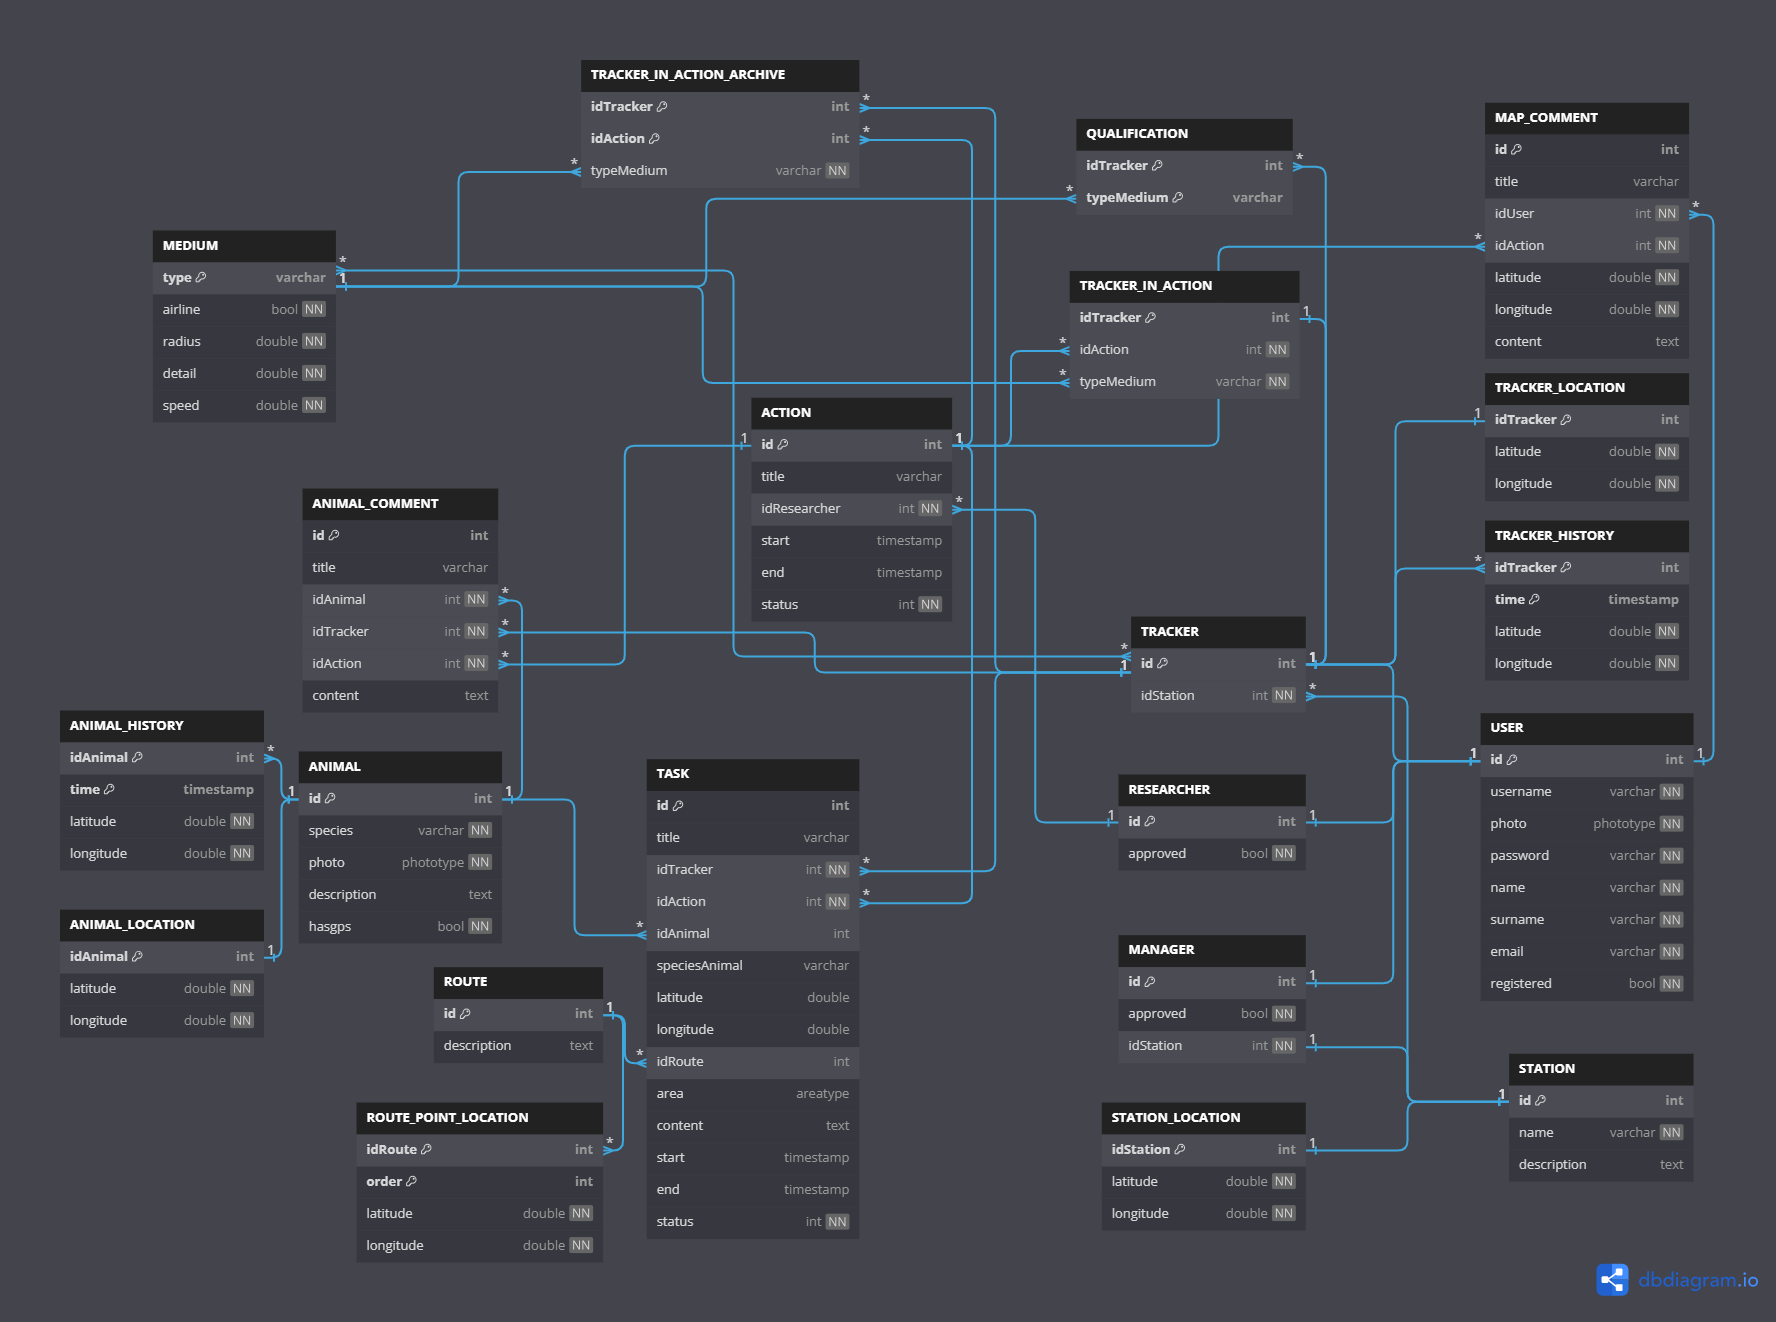
\includegraphics[scale=0.3]{slike/grafBaza.PNG} 
					% width=\textwidth,height=\textheight,keepaspectratio
					\centering
					\caption{E-R dijagram baze podataka}
					\label{fig:ERdiagram}
				\end{figure}				
				\restoregeometry
				
			\fi			
										
			
			\subsection{Dijagram baze podataka}			
			
				\vspace{12pt}						
				
				\begin{figure}[H] %ht
					\centering
					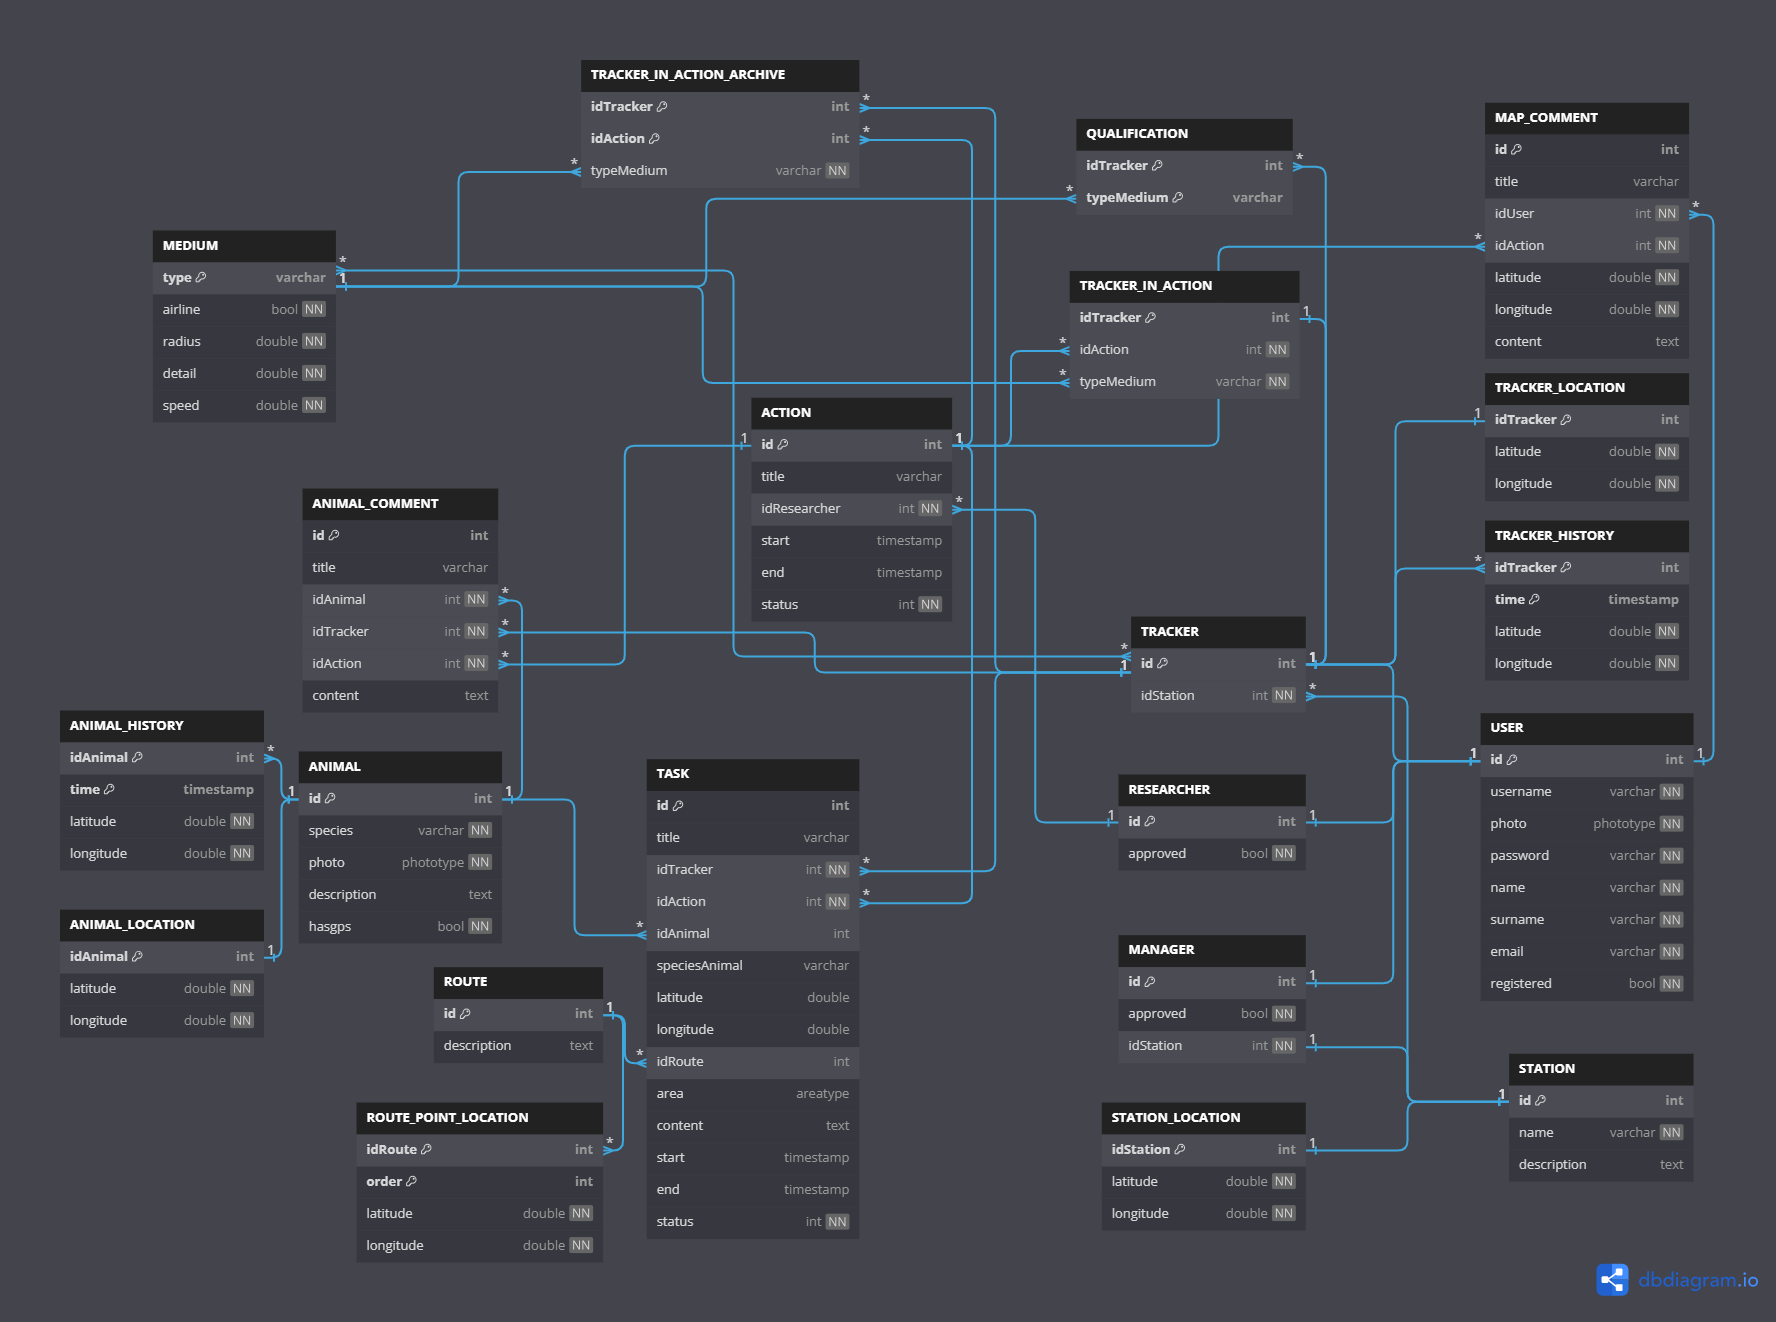
\includegraphics[width=\textwidth]{slike/grafBaza.PNG}
					\caption{E-R dijagram baze podataka}
					\label{fig:ERdiagram}
				\end{figure}																												
																																	
			\eject
						
			
			
		\section{Dijagram razreda}
		
			\textit{Potrebno je priložiti dijagram razreda s pripadajućim opisom. Zbog preglednosti je moguće dijagram razlomiti na više njih, ali moraju biti grupirani prema sličnim razinama apstrakcije i srodnim funkcionalnostima.}\\
			
			\textbf{\textit{dio 1. revizije}}\\
			
			\textit{Prilikom prve predaje projekta, potrebno je priložiti potpuno razrađen dijagram razreda vezan uz \textbf{generičku funkcionalnost} sustava. Ostale funkcionalnosti trebaju biti idejno razrađene u dijagramu sa sljedećim komponentama: nazivi razreda, nazivi metoda i vrste pristupa metodama (npr. javni, zaštićeni), nazivi atributa razreda, veze i odnosi između razreda.}\\
			
			\textbf{\textit{dio 2. revizije}}\\			
			
			\textit{Prilikom druge predaje projekta dijagram razreda i opisi moraju odgovarati stvarnom stanju implementacije}
			
			
			
			\eject
		
		\section{Dijagram stanja}
			
			
			\textbf{\textit{dio 2. revizije}}\\
			
			\textit{Potrebno je priložiti dijagram stanja i opisati ga. Dovoljan je jedan dijagram stanja koji prikazuje \textbf{značajan dio funkcionalnosti} sustava. Na primjer, stanja korisničkog sučelja i tijek korištenja neke ključne funkcionalnosti jesu značajan dio sustava, a registracija i prijava nisu. }
			
			
			\eject 
		
		\section{Dijagram aktivnosti}
			
			\textbf{\textit{dio 2. revizije}}\\
			
			 \textit{Potrebno je priložiti dijagram aktivnosti s pripadajućim opisom. Dijagram aktivnosti treba prikazivati značajan dio sustava.}
			
			\eject
		\section{Dijagram komponenti}
		
			\textbf{\textit{dio 2. revizije}}\\
		
			 \textit{Potrebno je priložiti dijagram komponenti s pripadajućim opisom. Dijagram komponenti treba prikazivati strukturu cijele aplikacije.}